\documentclass[12pt,a4paper]{report}

% ==========================================
% GÓI LỆNH VÀ CẤU HÌNH TRANG (THEO CHUẨN VIỆT NAM)
% ==========================================
\usepackage{fontspec}
\setmainfont{Times New Roman}
\setmonofont{Consolas}

\usepackage[left=3.0cm,right=2.0cm,top=2.0cm,bottom=2.0cm]{geometry}
\linespread{1.3} % Dãn dòng 1.3 theo Nghị định 30/2020/NĐ-CP

\usepackage{indentfirst}
\setlength{\parindent}{1.27cm} % Thụt đầu dòng 1.27cm (0.5 inch)
\setlength{\parskip}{6pt}      % Khoảng cách giữa các đoạn 6pt

\usepackage{amsmath,amssymb}
\usepackage{graphicx}
\usepackage{xcolor}
\usepackage{tabularx}
\usepackage{booktabs}
\usepackage{array}
\usepackage{fancyhdr}
\setlength{\headheight}{14.5pt}
\usepackage{titlesec}
\usepackage{tikz}
\usetikzlibrary{calc}
\usepackage{tcolorbox}
\usepackage{float}



% ==========================================
% CẤU HÌNH LIÊN KẾT VÀ MÀU SẮC
% ==========================================
\definecolor{navyblue}{RGB}{0, 32, 96}
\definecolor{darkblue}{RGB}{0, 51, 102}
\definecolor{codebg}{RGB}{248, 249, 250}
\definecolor{borderblue}{RGB}{0, 86, 179}
\definecolor{notebg}{RGB}{235, 243, 251}

\usepackage[unicode=true,bookmarks=true,bookmarksnumbered=true,bookmarksopen=true,linktoc=all]{hyperref}
\hypersetup{
    colorlinks=true,
    linkcolor=navyblue,
    filecolor=magenta,      
    urlcolor=blue,
    citecolor=blue,
    pdfauthor={Nguyễn Tấn Lộc},
    pdftitle={Báo cáo tự học: Authentication và Authorization trong ASP.NET Web Forms}
}



% ==========================================
% ĐỊNH DẠNG HEADER / FOOTER
% ==========================================
\pagestyle{fancy}
\fancyhf{}
\fancyhead[L]{\small\itshape Học phần: Lập trình Web ASPX}
\fancyhead[R]{\small\itshape Báo cáo giữa kỳ: Authentication \& Authorization}
\fancyfoot[C]{\thepage}
\renewcommand{\headrulewidth}{0.5pt}

% ==========================================
% ĐỊNH DẠNG TIÊU ĐỀ THEO CHUẨN NGHỊ ĐỊNH 30
% ==========================================
\titleformat{\chapter}[display]
  {\normalfont\bfseries\centering\color{navyblue}}
  {\Large\MakeUppercase{\chaptertitlename\ \thechapter}}
  {10pt}{\LARGE\MakeUppercase}
\titlespacing*{\chapter}{0pt}{-20pt}{20pt}

\titleformat{\section}
  {\normalfont\Large\bfseries\color{darkblue}}
  {\thesection}{1em}{}
\titlespacing*{\section}{0pt}{16pt}{8pt}

\titleformat{\subsection}
  {\normalfont\large\bfseries\itshape\color{black}}
  {\thesubsection}{1em}{}
\titlespacing*{\subsection}{0pt}{12pt}{6pt}

\titleformat{\subsubsection}
  {\normalfont\normalsize\bfseries\color{black}}
  {\thesubsubsection}{1em}{}
\titlespacing*{\subsubsection}{0pt}{8pt}{4pt}

% ==========================================
% CẤU HÌNH LISTINGS CHO MÃ NGUỒN C#, SQL, ASPX
% ==========================================
\usepackage{listings}
\lstset{
    backgroundcolor=\color{codebg},
    basicstyle=\ttfamily\footnotesize,
    breaklines=true,
    captionpos=b,
    frame=single,
    rulecolor=\color{borderblue},
    numbers=left,
    numberstyle=\tiny\color{gray},
    numbersep=7pt,
    tabsize=2,
    showstringspaces=false,
    keywordstyle=\color{blue}\bfseries,
    commentstyle=\color{green!50!black}\itshape,
    stringstyle=\color{red!70!black},
    escapeinside={\%*}{*)}
}

\renewcommand{\contentsname}{MỤC LỤC}
\renewcommand{\tablename}{Bảng}
\renewcommand{\figurename}{Hình}
\renewcommand{\listtablename}{DANH MỤC BẢNG BIỂU}
\renewcommand{\listfigurename}{DANH MỤC HÌNH ẢNH}

\begin{document}

% ==========================================
% TRANG BÌA CHÍNH QUY (COVER PAGE)
% ==========================================
\begin{titlepage}
\thispagestyle{empty}

\begin{tikzpicture}[remember picture, overlay]
  \draw[line width = 2pt, color = navyblue] 
    ($(current page.north west) + (2.5cm,-2.0cm)$) 
    rectangle 
    ($(current page.south east) + (-1.5cm,2.0cm)$);
  \draw[line width = 0.8pt, color = navyblue] 
    ($(current page.north west) + (2.65cm,-2.15cm)$) 
    rectangle 
    ($(current page.south east) + (-1.65cm,2.15cm)$);
\end{tikzpicture}

\begin{center}
    \vspace*{-0.5cm}
    \textbf{\large TRƯỜNG ĐẠI HỌC ĐỒNG THÁP}\\[0.2cm]
    \textbf{\large KHOA CÔNG NGHỆ VÀ KỸ THUẬT}\\[0.4cm]
    \rule{4.0cm}{0.8pt}\\[0.8cm]

    
\includegraphics[height=3.2cm]{logokonen.png}\\[1.0cm]

    \textbf{\LARGE\color{navyblue} BÁO CÁO TỰ HỌC}\\[0.4cm]
    \textbf{\large HỌC PHẦN: LẬP TRÌNH WEB ASPX}\\[0.9cm]

    \textit{\large Đề tài:}\\[0.35cm]
    \textbf{\large\color{navyblue} XÂY DỰNG HỆ THỐNG XÁC THỰC VÀ PHÂN QUYỀN TRUY CẬP}\\[0.25cm]
    \textbf{\large\color{navyblue} TRÊN NỀN TẢNG ASP.NET WEB FORMS VỚI SQL SERVER}\\[0.25cm]
    \textbf{\large\color{navyblue} (AUTHENTICATION \& AUTHORIZATION)}\\[1.4cm]

    \begin{flushleft}
    \hspace{1.5cm}
    \begin{tabular}{ll}
        \textbf{Giảng viên hướng dẫn:} & ThS. Trần Kim Hương \\[0.25cm]
        \textbf{Lớp:}                 & ĐHCNTT24B-IT \\[0.25cm]
        \textbf{Nhóm thực hiện:}       & Nhóm 6 \\[0.25cm]
        \textbf{Sinh viên thực hiện:}  & Nguyễn Tấn Lộc – MSSV: 0024417501 (Nhóm trưởng) \\[0.2cm]
                                       & Nguyễn Hoàng Thuận – MSSV: 0024418123 \\[0.2cm]
                                       & Phan Trần Gia Hưng – MSSV: 0024417689 \\[0.2cm]
                                       & Trần Ánh Dương – MSSV: 0024415950 \\[0.2cm]
                                       & Nguyễn Lê Phúc Thịnh – MSSV: 0024416432 \\
    \end{tabular}
    \end{flushleft}

    \vfill
    \textit{\large Đồng Tháp, tháng 11 năm 2026}\\[0.3cm]
\end{center}
\end{titlepage}

% ==========================================
% PHẦN ĐẦU TÀI LIỆU (LA MÃ: i, ii, iii...)
% ==========================================
\pagenumbering{roman}
\setcounter{page}{1}

\tableofcontents
\newpage

% ==========================================
% DANH MỤC TỪ VIẾT TẮT
% ==========================================
\chapter*{DANH MỤC TỪ VIẾT TẮT}
\addcontentsline{toc}{chapter}{DANH MỤC TỪ VIẾT TẮT}
\vspace*{-1.0cm}

\begin{center}
\small
\renewcommand{\arraystretch}{1.05}
\begin{tabularx}{\textwidth}{>{\raggedright\arraybackslash}p{2.3cm} >{\raggedright\arraybackslash}p{4.5cm} >{\raggedright\arraybackslash}X}
\toprule
\textbf{Từ viết tắt} & \textbf{Thuật ngữ tiếng Anh} & \textbf{Giải nghĩa tiếng Việt} \\
\midrule
\textbf{ASPX} & Active Server Pages Extended & Phần mở rộng trang web động của công nghệ ASP.NET \\
\textbf{AuthN} & Authentication & Xác thực danh tính người dùng (Bạn là ai?) \\
\textbf{AuthZ} & Authorization & Phân quyền truy cập và chức năng (Bạn được làm gì?) \\
\textbf{BFCache} & Back/Forward Cache & Bộ nhớ đệm rã đông trang tức thì khi bấm Back/Forward \\
\textbf{CRUD} & Create, Read, Update, Delete & Thao tác dữ liệu: Thêm, Đọc, Cập nhật, Xóa \\
\textbf{DDL} & Data Definition Language & Ngôn ngữ định nghĩa dữ liệu (CREATE, ALTER, DROP) \\
\textbf{DML} & Data Manipulation Language & Ngôn ngữ thao tác dữ liệu (SELECT, INSERT, UPDATE, DELETE) \\
\textbf{HTTP} & HyperText Transfer Protocol & Giao thức truyền tải siêu văn bản (phi trạng thái) \\
\textbf{IDE} & Integrated Development Environment & Môi trường phát triển tích hợp (Visual Studio) \\
\textbf{JWT} & JSON Web Token & Chuẩn mã hóa thông tin xác thực dạng chuỗi Token JSON \\
\textbf{RBAC} & Role-Based Access Control & Mô hình kiểm soát truy cập dựa trên vai trò người dùng \\
\textbf{RDBMS} & Relational Database Management System & Hệ quản trị cơ sở dữ liệu quan hệ \\
\textbf{SQL} & Structured Query Language & Ngôn ngữ truy vấn có cấu trúc \\
\textbf{SQLi} & SQL Injection & Hình thức tấn công chèn mã độc vào câu lệnh truy vấn SQL \\
\textbf{SSMS} & SQL Server Management Studio & Công cụ quản trị cơ sở dữ liệu Microsoft SQL Server \\
\textbf{UI / UX} & User Interface / User Experience & Giao diện người dùng / Trải nghiệm người dùng \\
\bottomrule
\end{tabularx}
\end{center}
\newpage

% ==========================================
% DANH MỤC BẢNG BIỂU
% ==========================================
\chapter*{DANH MỤC BẢNG BIỂU}
\addcontentsline{toc}{chapter}{DANH MỤC BẢNG BIỂU}
\vspace*{-0.5cm}

\begin{center}
\renewcommand{\arraystretch}{1.25}
\begin{tabularx}{\textwidth}{>{\raggedright\arraybackslash}p{2.5cm} >{\raggedright\arraybackslash}X >{\raggedleft\arraybackslash}p{2.0cm}}
\toprule
\textbf{Ký hiệu} & \textbf{Tên bảng biểu mô tả} & \textbf{Trang} \\
\midrule
\hyperref[tab:ss_vs_forms_jwt]{\textbf{Bảng 1.1}} & \hyperref[tab:ss_vs_forms_jwt]{So sánh chi tiết giữa Session State, Forms Authentication và JWT Token} & \pageref{tab:ss_vs_forms_jwt} \\
\addlinespace
\hyperref[tab:nguoidung_schema]{\textbf{Bảng 2.1}} & \hyperref[tab:nguoidung_schema]{Đặc tả cấu trúc bảng dữ liệu NguoiDung trong CSDL QL\_NguoiDung} & \pageref{tab:nguoidung_schema} \\
\addlinespace
\hyperref[tab:rubric_danhgia]{\textbf{Bảng 2.2}} & \hyperref[tab:rubric_danhgia]{Tiêu chí đánh giá và Rubric chấm điểm bài thực hành phân quyền 5 tiết} & \pageref{tab:rubric_danhgia} \\
\addlinespace
\hyperref[tab:test_cases]{\textbf{Bảng 2.3}} & \hyperref[tab:test_cases]{Kết quả kiểm thử an ninh 5 kịch bản thực tế} & \pageref{tab:test_cases} \\
\bottomrule
\end{tabularx}
\end{center}
\newpage

% ==========================================
% DANH MỤC HÌNH ẢNH
% ==========================================
\chapter*{DANH MỤC HÌNH ẢNH}
\addcontentsline{toc}{chapter}{DANH MỤC HÌNH ẢNH}
\vspace*{-0.5cm}

\begin{center}
\renewcommand{\arraystretch}{1.25}
\begin{tabularx}{\textwidth}{>{\raggedright\arraybackslash}p{2.5cm} >{\raggedright\arraybackslash}X >{\raggedleft\arraybackslash}p{2.0cm}}
\toprule
\textbf{Ký hiệu} & \textbf{Tên hình ảnh mô tả} & \textbf{Trang} \\
\midrule
\hyperref[fig:csdl_nguoidung]{\textbf{Hình 2.1}} & \hyperref[fig:csdl_nguoidung]{Dữ liệu thực tế của bảng NguoiDung trong SQL Server} & \pageref{fig:csdl_nguoidung} \\
\addlinespace
\hyperref[fig:so_do_dieu_huong]{\textbf{Hình 2.2}} & \hyperref[fig:so_do_dieu_huong]{Sơ đồ luồng điều hướng và kiểm soát truy cập hệ thống Login + Role} & \pageref{fig:so_do_dieu_huong} \\
\addlinespace
\hyperref[fig:ui_login]{\textbf{Hình 2.3}} & \hyperref[fig:ui_login]{Giao diện trang Đăng nhập hệ thống (Login.aspx)} & \pageref{fig:ui_login} \\
\addlinespace
\hyperref[fig:ui_admin]{\textbf{Hình 2.4}} & \hyperref[fig:ui_admin]{Giao diện trang Quản trị (Admin.aspx) với quyền hạn Admin và bảng Repeater} & \pageref{fig:ui_admin} \\
\addlinespace
\hyperref[fig:ui_user]{\textbf{Hình 2.5}} & \hyperref[fig:ui_user]{Giao diện Cổng thông tin người dùng (User.aspx) ở chế độ Chỉ xem (Read-only)} & \pageref{fig:ui_user} \\
\addlinespace
\hyperref[fig:ui_accessdenied]{\textbf{Hình 2.6}} & \hyperref[fig:ui_accessdenied]{Giao diện trang cảnh báo Từ chối truy cập 403 Forbidden (AccessDenied.aspx)} & \pageref{fig:ui_accessdenied} \\
\bottomrule
\end{tabularx}
\end{center}
\newpage



% ==========================================
% BẮT ĐẦU NỘI DUNG CHÍNH (SỐ TRANG 1, 2, 3...)
% ==========================================
\pagenumbering{arabic}
\setcounter{page}{1}

% ==========================================
% CHƯƠNG 1
% ==========================================
\chapter{CƠ SỞ LÝ THUYẾT VỀ XÁC THỰC VÀ PHÂN QUYỀN}

\section{Tổng quan về nền tảng ASP.NET Web Forms}

\subsection{Kiến trúc và mô hình lập trình hướng sự kiện (Event-Driven Programming)}
ASP.NET Web Forms là một mô hình phát triển ứng dụng web dựa trên máy chủ (server-side web framework) thuộc hệ sinh thái .NET Framework do Microsoft phát triển. Mục tiêu cốt lõi của Web Forms khi ra đời là trừu tượng hóa và che giấu sự phức tạp vốn có của giao thức truyền tải siêu văn bản (HTTP) -- một giao thức có bản chất phi trạng thái (stateless protocol). Thông qua cơ chế trừu tượng này, các lập trình viên đã quen thuộc với việc phát triển ứng dụng máy trạm (Desktop GUI như Windows Forms, WPF) có thể dễ dàng chuyển đổi sang xây dựng các hệ thống web tương tác nghiệp vụ cao mà không cần trực tiếp thao tác với mã JavaScript thô hay xử lý thủ công các truy vấn HTTP request/response ở tầng thấp.

Trong kiến trúc Web Forms, toàn bộ tương tác của người dùng được mô hình hóa theo phong cách lập trình hướng sự kiện (Event-Driven Programming). Giao diện người dùng được cấu thành từ hệ sinh thái các điều khiển máy chủ (Server Controls) như \texttt{asp:TextBox}, \texttt{asp:Button}, \texttt{asp:Repeater}, \texttt{asp:Label}. Khi người dùng cuối kích hoạt một tương tác trên trình duyệt (chẳng hạn như nhấn nút Đăng nhập hoặc bấm nút Xóa dữ liệu), trình duyệt sẽ gửi một yêu cầu HTTP POST về lại máy chủ web (gọi là PostBack), từ đó kích hoạt các phương thức xử lý sự kiện phía sau (như \texttt{btnLogin\_Click}, \texttt{Page\_Load}) được viết bằng ngôn ngữ C\#.

Để đảm bảo nguyên tắc phân tách trách nhiệm (Separation of Concerns), mỗi trang web trong ASP.NET Web Forms luôn bao gồm một cặp tệp song hành:
\begin{itemize}
    \item \textbf{Tệp giao diện (.aspx):} Chứa mã đánh dấu HTML kết hợp với các thẻ điều khiển máy chủ của ASP.NET (được nhận dạng qua thuộc tính \texttt{runat="server"}). Tệp này định nghĩa cấu trúc trình diễn và bố cục của trang web.
    \item \textbf{Tệp mã xử lý phía sau (Code-Behind .aspx.cs):} Chứa mã nguồn C\# thực thi logic nghiệp vụ, kết nối cơ sở dữ liệu, kiểm tra quyền hạn và phản hồi các sự kiện. Hai tệp này được liên kết chặt chẽ thông qua cơ chế lớp riêng một phần (\textit{partial class}) của C\#, cho phép mã C\# truy xuất trực tiếp các phần tử giao diện thông qua thuộc tính định danh (ID).
\end{itemize}

\subsection{Bản chất phi trạng thái của HTTP và cơ chế quản lý trạng thái (State Management)}
Giao thức HTTP vận hành theo mô hình yêu cầu -- phản hồi (Request -- Response) độc lập: Sau khi máy chủ gửi dữ liệu phản hồi về trình duyệt, kết nối mạng sẽ bị đóng lại ngay lập tức. Máy chủ web hoàn toàn không lưu giữ bất kỳ ký ức nào về việc người dùng đó là ai, đã đăng nhập thành công hay chưa, hoặc trạng thái của các ô nhập liệu ở các lượt truy cập trước đó. Đây chính là thách thức căn bản khi xây dựng các hệ thống đòi hỏi tính liên tục như Cổng thông tin nội bộ, Hệ thống quản trị (Admin Panel), hay Giỏ hàng thương mại điện tử.

Để khắc phục bản chất phi trạng thái này, ASP.NET Web Forms cung cấp cơ chế Quản lý trạng thái (State Management) đa tầng, được chia thành hai nhóm chính:
\begin{enumerate}
    \item \textbf{Quản lý trạng thái phía máy khách (Client-Side State Management):} Bao gồm ViewState, Hidden Field, Cookie, QueryString. Trong đó, ViewState nén toàn bộ trạng thái điều khiển trên form thành chuỗi mã hóa Base64 và nhúng ngầm vào trường ẩn \texttt{\_\_VIEWSTATE} trong mã HTML.
    \item \textbf{Quản lý trạng thái phía máy chủ (Server-Side State Management):} Bao gồm Application State, Cache và Session State. Trong đó, Session State là cơ chế trọng yếu nhất được sử dụng để quản lý thông tin phiên làm việc của từng người dùng riêng biệt trên bộ nhớ RAM của máy chủ web.
\end{enumerate}

\subsection{Vòng đời trang (Page Lifecycle) và cơ chế gửi ngược (PostBack)}
Mỗi khi một yêu cầu trang .aspx được gửi tới máy chủ IIS/ASP.NET, trang web sẽ trải qua một chuỗi các giai đoạn tuần tự nghiêm ngặt gọi là Vòng đời trang (Page Lifecycle). Việc nắm vững vòng đời trang là chìa khóa then chốt để lập trình viên đặt mã kiểm tra bảo mật đúng thời điểm, ngăn chặn mã độc thực thi trước khi được cấp phép:
\begin{itemize}
    \item \textbf{Giai đoạn Khởi tạo (Page\_Init):} Khởi tạo cây điều khiển (Control Tree) và thiết lập các thuộc tính ban đầu.
    \item \textbf{Giai đoạn Tải trạng thái (LoadViewState):} Phục hồi lại dữ liệu trạng thái của các điều khiển từ chuỗi \texttt{\_\_VIEWSTATE} gửi lên từ client.
    \item \textbf{Giai đoạn Tải trang (Page\_Load):} Phương thức \texttt{Page\_Load} trong Code-Behind được thực thi. \textbf{ĐÂY LÀ ĐỊA ĐIỂM CHIẾN LƯỢC ĐỂ THỰC HIỆN KIỂM TRA BẢO MẬT (Authentication \& Authorization).} Nếu phát hiện người dùng chưa đăng nhập hoặc không đủ quyền hạn, hệ thống phải thực hiện chuyển hướng ngay lập tức (\texttt{Response.Redirect}) và dừng hàm bằng lệnh \texttt{return} để bảo vệ các logic nạp dữ liệu bên dưới.
    \item \textbf{Giai đoạn Xử lý sự kiện điều khiển (Control Events):} Kích hoạt các sự kiện người dùng bấm (như \texttt{btnLogin\_Click}, \texttt{btnLogout\_Click}).
    \item \textbf{Giai đoạn Kết xuất (Render):} Máy chủ chuyển dịch toàn bộ cây Server Control thành mã HTML thuần túy và đẩy về trình duyệt.
    \item \textbf{Giai đoạn Giải phóng (Unload):} Hủy bỏ các đối tượng kết nối CSDL và giải phóng bộ nhớ RAM.
\end{itemize}

Trong vòng đời này, thuộc tính \texttt{IsPostBack} đóng vai trò phân biệt: Ở lần tải trang đầu tiên (người dùng gõ URL hoặc bấm link), \texttt{IsPostBack} có giá trị \texttt{false}. Ở các lần bấm nút thao tác gửi ngược dữ liệu, \texttt{IsPostBack} có giá trị \texttt{true}. Lập trình viên luôn bọc các hàm nạp dữ liệu ban đầu trong khối \texttt{if (!IsPostBack)} để tránh việc dữ liệu bị nạp đè trùng lặp ở mỗi lần tương tác.

\section{Lý thuyết về Xác thực và Phân quyền (Authentication \& Authorization)}

\subsection{Khái niệm và sự khác biệt bản chất giữa Authentication và Authorization}
Trong lĩnh vực an toàn thông tin và kiến trúc phần mềm doanh nghiệp, Xác thực (Authentication) và Phân quyền (Authorization) là hai khái niệm cốt lõi nhưng thường bị nhầm lẫn. Hệ thống cần thực hiện chặt chẽ cả hai cơ chế theo đúng thứ tự logic:
\begin{enumerate}
    \item \textbf{Authentication (Xác thực danh tính -- AuthN):} Giải quyết câu hỏi cốt lõi: \textit{“BẠN LÀ AI?”}. Đây là quá trình thẩm định và xác minh danh tính được tuyên bố của người dùng. Người dùng cung cấp thông tin định danh (Tên đăng nhập) cùng bằng chứng chứng minh danh tính (Mật khẩu). Hệ thống đối chiếu với Cơ sở dữ liệu; nếu thông tin trùng khớp, hệ thống công nhận danh tính và cấp một định danh phiên (Session) hợp lệ.
    \item \textbf{Authorization (Cấp phép truy cập -- AuthZ):} Giải quyết câu hỏi cốt lõi: \textit{“BẠN ĐƯỢC PHÉP LÀM GÌ?”}. Quá trình này LUÔN DIỄN RA SAU Authentication. Sau khi đã biết rõ người dùng là ai, hệ thống tiếp tục kiểm tra quyền hạn (Role / Permissions) của người đó để quyết định: Người này có được phép truy cập vào trang Quản trị (\texttt{Admin.aspx}) hay không? Có được quyền thực hiện các thao tác phá hủy dữ liệu (Sửa, Xóa) hay không? Nếu người dùng cố tình truy cập vào tài nguyên vượt quá thẩm quyền của mình, hệ thống sẽ chặn đứng và trả về thông báo lỗi 403 Forbidden (Từ chối truy cập).
\end{enumerate}

\subsection{Mô hình kiểm soát truy cập dựa trên vai trò (Role-Based Access Control - RBAC)}
RBAC (Role-Based Access Control) là mô hình chuẩn mực và phổ biến nhất trong các hệ thống phần mềm doanh nghiệp. Thay vì gán trực tiếp hàng chục quyền hạn rời rạc cho từng người dùng riêng lẻ (rất dễ gây nhầm lẫn và khó quản lý), hệ thống nhóm các quyền hạn vào các Vai trò (Roles). Người dùng được gán vào các vai trò tương ứng với trách nhiệm công việc của họ.

Trong phạm vi đề tài này, hệ thống thiết kế mô hình RBAC 2 cấp độ phân minh rõ ràng:
\begin{itemize}
    \item \textbf{Vai trò Quản trị viên (Role: Admin):} Được trao toàn quyền trong hệ thống, bao gồm quyền đăng nhập, xem danh sách, thêm mới, chỉnh sửa thông tin, và xóa bản ghi trên trang quản trị chuyên biệt (\texttt{Admin.aspx}).
    \item \textbf{Vai trò Người dùng thông thường (Role: User):} Chỉ được cấp quyền đọc dữ liệu dạng tra cứu (Read-only) trên Cổng thông tin (\texttt{User.aspx}), hoàn toàn không được phép truy cập vào trang Admin hay nhìn thấy các nút chức năng quản trị.
\end{itemize}

\subsection{Quản lý phiên làm việc bằng Session State và Cookie ASP.NET\_SessionId}
Vì giao thức HTTP là phi trạng thái, ASP.NET Web Forms giải quyết bài toán duy trì phiên làm việc cho từng người dùng thông qua cơ chế Stateful Session (Quản lý phiên trạng thái trên máy chủ):
\begin{enumerate}
    \item Khi người dùng gửi yêu cầu đầu tiên, máy chủ ASP.NET tự động sinh ra một chuỗi định danh ngẫu nhiên dài 24 ký tự có tên là \texttt{ASP.NET\_SessionId}. Chuỗi này được gửi về lưu trữ tại trình duyệt của người dùng dưới dạng một Cookie phiên (Session Cookie).
    \item Khi người dùng thực hiện Đăng nhập thành công, máy chủ lưu các thông tin nhạy cảm (như Tên đăng nhập, Quyền hạn) vào một vùng nhớ RAM riêng biệt trên máy chủ tương ứng với SessionId đó: \texttt{Session["Username"] = username; Session["Role"] = quyen;}.
    \item Ở các yêu cầu tiếp theo đến các trang nội bộ (\texttt{Admin.aspx} hay \texttt{User.aspx}), trình duyệt tự động đính kèm Cookie \texttt{ASP.NET\_SessionId} lên máy chủ. Máy chủ tìm vùng nhớ RAM tương ứng để đọc lại quyền hạn của người dùng mà không bắt họ phải gõ lại mật khẩu.
    \item \textbf{Ưu điểm bảo mật vượt trội:} Toàn bộ thông tin định danh và quyền hạn (Admin/User) ĐƯỢC LƯU TRỮ HOÀN TOÀN TRÊN RAM CỦA MÁY CHỦ, người dùng ở phía Client chỉ cầm chìa khóa ngẫu nhiên (SessionId) nên không thể dùng công cụ trình duyệt để tự sửa đổi quyền hạn của mình.
\end{enumerate}

\subsection{Phân tích 5 nguy cơ tấn công và lỗ hổng truy cập trái phép phổ biến}
Trong quá trình xây dựng hệ thống web, nếu chỉ dựa vào giao diện thông thường mà không có các lớp kiểm soát bảo mật chặt chẽ ở tầng mã nguồn máy chủ, hệ thống sẽ đối mặt với 5 nguy cơ tấn công nguy hiểm sau:
\begin{itemize}
    \item \textbf{Nguy cơ 1 (Force Browsing):} Kẻ tấn công không cần đăng nhập nhưng tự ý gõ thẳng địa chỉ trang quản trị (\texttt{http://localhost/Admin.aspx}) vào thanh URL trình duyệt để xem trộm dữ liệu.
    \item \textbf{Nguy cơ 2 (Privilege Escalation):} Người dùng quyền User bình thường cố tình sửa địa chỉ trên trình duyệt từ \texttt{User.aspx} thành \texttt{Admin.aspx} nhằm chiếm đoạt quyền quản lý của Admin.
    \item \textbf{Nguy cơ 3 (SQL Injection):} Kẻ tấn công chèn các chuỗi cú pháp SQL độc hại (như \texttt{admin' --} hoặc \texttt{' OR 1=1 --}) vào ô đăng nhập nhằm bẻ gãy câu lệnh SQL để đăng nhập mà không cần mật khẩu.
    \item \textbf{Nguy cơ 4 (Browser Cache / BFCache Snooping):} Sau khi Quản trị viên bấm Đăng xuất, người sau ngồi vào máy bấm nút Back trên trình duyệt và thấy lại toàn bộ dữ liệu do bộ nhớ đệm BFCache của trình duyệt lưu trữ.
    \item \textbf{Nguy cơ 5 (DOM Tampering via F12):} Người dùng quyền User mở công cụ Developer Tools (F12) trên trình duyệt để sửa mã HTML, bỏ thuộc tính disabled của các nút thao tác hoặc gửi các yêu cầu PostBack giả mạo.
\end{itemize}

\section{Các điều khiển Web Forms sử dụng trong hệ thống}

\subsection{Cơ chế liên kết dữ liệu (Data Binding) và điều khiển Repeater}
Liên kết dữ liệu (Data Binding) trong Web Forms là quy trình gắn kết dữ liệu từ một tập hợp (DataTable, List$<$T$>$) với một điều khiển giao diện lặp. Trong khi điều khiển GridView thường tự động sinh ra mã bảng với các thuộc tính mặc định cồng kềnh, điều khiển \texttt{asp:Repeater} được lựa chọn trong dự án này vì mang lại khả năng tùy biến giao diện cao nhất:
\begin{itemize}
    \item Repeater không tự động sinh ra bất kỳ thẻ HTML bao ngoài nào, cho phép lập trình viên toàn quyền kiểm soát mã HTML, dễ dàng kết hợp với các lớp CSS hiện đại của Bootstrap 5 (\texttt{table}, \texttt{table-hover}, \texttt{table-striped}, \texttt{badge}).
    \item Cấu trúc Repeater bao gồm: \texttt{<HeaderTemplate>} định nghĩa tiêu đề bảng, \texttt{<ItemTemplate>} định nghĩa từng dòng dữ liệu thông qua cú pháp đánh giá \texttt{<\%\# Eval("TenTruong") \%>}, và \texttt{<FooterTemplate>} đóng thẻ bảng.
    \item Quy trình thực thi gồm 2 bước trong Code-Behind: Gán nguồn dữ liệu (\texttt{rptNguoiDung.DataSource = dt}) và kích hoạt hiển thị (\texttt{rptNguoiDung.DataBind()}).
\end{itemize}

\subsection{Điều khiển kiểm tra hợp lệ dữ liệu (RequiredFieldValidator)}
Điều khiển \texttt{asp:RequiredFieldValidator} được sử dụng trên form đăng nhập để đảm bảo người dùng không để trống tên đăng nhập hoặc mật khẩu. Ưu điểm lớn của điều khiển này là cung cấp cơ chế kiểm tra tính hợp lệ kép (Double Validation): Ở phía Client, tự động chặn form submit nếu rỗng; ở phía Server, kiểm tra lại thông qua \texttt{Page.IsValid} trước khi thực thi truy vấn SQL.

\section{So sánh chuyên sâu: Quản lý phiên bằng Session State, Forms Authentication và JWT Token}
Bảng dưới đây tiến hành phân tích và so sánh chi tiết giữa 3 công nghệ xác thực phổ biến:

\begin{table}[H]
\centering
\small
\renewcommand{\arraystretch}{1.2}
\begin{tabularx}{\textwidth}{>{\raggedright\arraybackslash}p{3.2cm} >{\raggedright\arraybackslash}X >{\raggedright\arraybackslash}X >{\raggedright\arraybackslash}X}
\toprule
\textbf{Tiêu chí so sánh} & \textbf{Session State (Đề tài)} & \textbf{Forms Authentication} & \textbf{Token-based (JWT)} \\
\midrule
\textbf{Vị trí lưu trữ dữ liệu phiên} & 100\% trên bộ nhớ RAM của Web Server & Mã hóa trong Cookie máy khách (.ASPXAUTH) & Mã hóa trong chuỗi Token trên Client (LocalStorage/Cookie) \\
\addlinespace
\textbf{Mức độ phức tạp \& Triển khai} & Đơn giản, dễ học, tích hợp sẵn, phù hợp tuyệt đối cho môn học Web Forms & Trung bình, cấu hình qua file Web.config và web.sitemap & Phức tạp, đòi hỏi xử lý chữ ký HMAC/RSA, Token Refresh và CORS \\
\addlinespace
\textbf{Mức độ an toàn thông tin} & Rất cao (Client chỉ giữ ID ngẫu nhiên, không thể giả mạo dữ liệu quyền hạn) & Khá (Nếu lộ khóa MachineKey có thể bị giải mã Cookie) & Rất cao nếu dùng HttpOnly Cookie, nhưng dễ bị XSS nếu lưu trong LocalStorage \\
\addlinespace
\textbf{Khả năng mở rộng (Scale)} & Giới hạn khi chạy nhiều Server (cần dùng SQL Server Session State) & Tốt nếu dùng chung MachineKey giữa các Server & Xuất sắc, hoàn toàn Stateless, tối ưu cho Microservices và App di động \\
\addlinespace
\textbf{Quản lý Đăng xuất (Logout)} & Lập tức hủy bỏ trên Server (\texttt{Session.Abandon()}), an toàn tức thì & Xóa Cookie trên Client (\texttt{FormsAuth.SignOut()}) & Khó thu hồi Token trước hạn (cần cơ chế Blacklist/Redis) \\
\addlinespace
\textbf{Phù hợp ngữ cảnh nào} & Hệ thống quản trị nội bộ doanh nghiệp, đồ án sinh viên, trường học & Hệ thống Web Forms truyền thống đa trang & Single Page App (React/Vue/Angular), Mobile App, RESTful API \\
\bottomrule
\end{tabularx}
\caption{So sánh chi tiết giữa Session State, Forms Authentication và JWT Token}\label{tab:ss_vs_forms_jwt}
\end{table}

% ==========================================
% CHƯƠNG 2
% ==========================================
\chapter{HƯỚNG DẪN THỰC HÀNH XÂY DỰNG HỆ THỐNG PHÂN QUYỀN QL\_NGUOIDUNG}

\section{Phân tích bài toán và thiết kế cơ sở dữ liệu trên SQL Server}
Bài toán đặt ra là xây dựng một cổng thông tin xác thực tập trung cho một tổ chức giáo dục / doanh nghiệp. Hệ thống yêu cầu phân định rạch ròi giữa hai nhóm đối tượng: Quản trị viên (Admin) -- người chịu trách nhiệm quản lý danh sách người dùng, và Người dùng thông thường (User) -- người chỉ có quyền tra cứu thông tin cá nhân và danh bạ thành viên.

Cơ sở dữ liệu QL\_NguoiDung được thiết kế trên hệ quản trị Microsoft SQL Server với bảng trung tâm \texttt{NguoiDung} có cấu trúc chuẩn hóa như sau:

\begin{table}[H]
\centering
\footnotesize
\setlength{\tabcolsep}{3.5pt}
\renewcommand{\arraystretch}{1.02}
\begin{tabularx}{\textwidth}{>{\raggedright\arraybackslash}p{2.2cm} >{\raggedright\arraybackslash}p{2.6cm} >{\raggedright\arraybackslash}p{2.5cm} >{\raggedright\arraybackslash}X >{\raggedright\arraybackslash}p{3.2cm}}
\toprule
\textbf{Tên cột} & \textbf{Kiểu dữ liệu} & \textbf{Khóa / Ràng buộc} & \textbf{Mô tả nghiệp vụ} & \textbf{Ghi chú an ninh} \\
\midrule
\texttt{Id} & INT & PRIMARY KEY,\newline IDENTITY(1,1) & Mã định danh duy nhất của người dùng & Khóa chính tự tăng, bất biến \\
\texttt{TenDangNhap} & VARCHAR(50) & NOT NULL, UNIQUE & Tên tài khoản đăng nhập hệ thống & Unique Index chống tạo trùng \\
\texttt{MatKhau} & VARCHAR(50) & NOT NULL & Mật khẩu xác thực đăng nhập & Cần mã hóa băm (Hash/Salt) \\
\texttt{HoTen} & NVARCHAR(100) & NOT NULL & Họ và tên đầy đủ hiển thị & Hỗ trợ Unicode Tiếng Việt \\
\texttt{Email} & VARCHAR(100) & NULL & Hòm thư điện tử liên hệ & Tra cứu danh bạ nội bộ \\
\texttt{Quyen} & VARCHAR(20) & NOT NULL & Quyền hạn: \textbf{'Admin'} hoặc \textbf{'User'} & Trọng tâm kiểm soát Authorization \\
\texttt{TrangThai} & NVARCHAR(30) & DEFAULT N'Đang hoạt động' & Trạng thái hoạt động tài khoản & Cho phép khóa/kích hoạt phiên \\
\bottomrule
\end{tabularx}
\caption{Đặc tả cấu trúc bảng dữ liệu NguoiDung trong CSDL QL\_NguoiDung}\label{tab:nguoidung_schema}
\end{table}

\begin{tcolorbox}[colback=notebg,colframe=borderblue,title=\textbf{ĐẶC TẢ NGHIỆP VỤ PHÂN QUYỀN}]
Trong bảng NguoiDung, trường \texttt{Quyen} mang tính quyết định đến luồng phân quyền (Authorization). Hệ thống chỉ chấp nhận hai giá trị chuẩn mực là \textbf{'Admin'} và \textbf{'User'}. Mọi truy vấn điều hướng và kiểm soát truy cập trên trang sẽ dựa trên giá trị của trường này khi được nạp vào bộ nhớ Session.
\end{tcolorbox}

Đoạn kịch bản SQL (\texttt{database.sql}) hoàn chỉnh để khởi tạo cơ sở dữ liệu và nạp dữ liệu mẫu thử nghiệm:

\begin{lstlisting}[language=SQL, caption={Kịch bản khởi tạo CSDL QL\_NguoiDung}]
-- 1. TAO CO SO DU LIEU
IF NOT EXISTS (SELECT * FROM sys.databases WHERE name = 'QL_NguoiDung')
BEGIN
    CREATE DATABASE QL_NguoiDung;
END
GO
USE QL_NguoiDung;
GO

-- 2. TAO BANG NGUOIDUNG VOI DAY DU RANG BUOC
IF NOT EXISTS (SELECT * FROM sys.tables WHERE name = 'NguoiDung')
BEGIN
    CREATE TABLE NguoiDung (
        Id INT IDENTITY(1,1) PRIMARY KEY,
        TenDangNhap VARCHAR(50) NOT NULL UNIQUE,
        MatKhau VARCHAR(50) NOT NULL,
        HoTen NVARCHAR(100) NOT NULL,
        Email VARCHAR(100),
        Quyen VARCHAR(20) NOT NULL, -- 'Admin' hoac 'User'
        TrangThai NVARCHAR(30) DEFAULT N'Dang hoat dong'
    );
END
GO

-- 3. NAP DU LIEU MAU DE TEST PHAN QUYEN
INSERT INTO NguoiDung (TenDangNhap, MatKhau, HoTen, Email, Quyen, TrangThai) VALUES
('admin', '123', N'Quan Tri Vien He Thong', 'admin@dthu.edu.vn', 'Admin', N'Dang hoat dong'),
('locadmin', '123', N'Nguyen Tan Loc (Admin)', 'tanloc@dthu.edu.vn', 'Admin', N'Dang hoat dong'),
('user', '123', N'Nguoi Dung Mau', 'user@dthu.edu.vn', 'User', N'Dang hoat dong'),
('giahung', '123', N'Phan Tran Gia Hung', 'giahung@dthu.edu.vn', 'User', N'Dang hoat dong'),
('vanan', '123', N'Tran Van An', 'vanan@dthu.edu.vn', 'User', N'Dang hoat dong'),
('thuhuong', '123', N'Le Thi Thu Huong', 'thuhuong@dthu.edu.vn', 'User', N'Dang hoat dong');
GO
\end{lstlisting}

\begin{figure}[H]
\centering
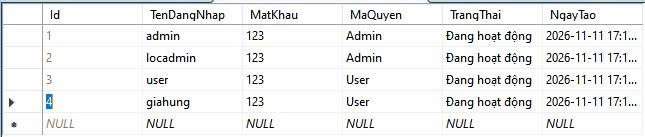
\includegraphics[width=0.88\textwidth]{hinh2_1_csdl_nguoidung.jpg}
\caption{Dữ liệu thực tế của bảng NguoiDung trong SQL Server Management Studio}\label{fig:csdl_nguoidung}
\end{figure}

\section{Khởi tạo dự án ASP.NET Web Forms và cấu hình Web.config}
Quy trình khởi tạo dự án trên phần mềm Microsoft Visual Studio 2022:
\begin{itemize}
    \item \textbf{Bước 1:} Mở Visual Studio $\rightarrow$ Chọn \textit{Create a new project}.
    \item \textbf{Bước 2:} Lọc ngôn ngữ C\#, nền tảng Windows, loại ứng dụng Web. Chọn mẫu \textit{ASP.NET Web Application (.NET Framework)} $\rightarrow$ Nhấn Next.
    \item \textbf{Bước 3:} Đặt tên dự án là \texttt{SEMI\_FINAL\_ASPX}, chọn .NET Framework 4.7.2 (hoặc 4.8) $\rightarrow$ Nhấn Create.
    \item \textbf{Bước 4:} Tại hộp thoại cấu hình, chọn mẫu Web Forms (hoặc Empty và tích chọn ô Web Forms) $\rightarrow$ Nhấn Create.
\end{itemize}

Cấu hình tệp \texttt{Web.config} là bước quan trọng nhất để thiết lập kết nối CSDL và xử lý hiển thị font chữ tiếng Việt toàn cục. Lập trình viên cần bổ sung chuỗi kết nối và cấu hình thẻ \texttt{globalization} như sau:

\begin{lstlisting}[language=XML, caption={Cấu hình chuỗi kết nối và Globalization trong Web.config}]
<configuration>
  <connectionStrings>
    <!-- Khai bao chuoi ket noi an toan toi SQL Server localhost -->
    <add name="QLNguoiDungConn" 
         connectionString="Data Source=localhost;Initial Catalog=QL_NguoiDung;Integrated Security=True" 
         providerName="System.Data.SqlClient" />
  </connectionStrings>

  <system.web>
    <!-- Cau hinh chuan ma hoa UTF-8 tieng Viet toan cuc, tranh loi font -->
    <globalization fileEncoding="utf-8" requestEncoding="utf-8" responseEncoding="utf-8" 
                   culture="vi-VN" uiCulture="vi-VN" />
    <compilation debug="true" targetFramework="4.7.2" />
    <httpRuntime targetFramework="4.7.2" />
  </system.web>
</configuration>
\end{lstlisting}

\section{Thiết kế giao diện người dùng hiện đại với Bootstrap 5}
Hệ thống bao gồm 4 trang giao diện độc lập được thiết kế đồng bộ theo phong cách hiện đại với thư viện Bootstrap 5:
\begin{enumerate}
    \item \textbf{Trang Đăng nhập (Login.aspx):} Thiết kế dạng Split-screen (chia đôi màn hình). Nửa bên trái là khối thương hiệu với dải màu Gradient (\#4f46e5 đến \#7c3aed) và logo học phần. Nửa bên phải là form đăng nhập gồm các ô \texttt{asp:TextBox}, thông báo lỗi \texttt{asp:Label} (màu đỏ) và các điều khiển \texttt{asp:RequiredFieldValidator} bắt lỗi bỏ trống.
    \item \textbf{Trang Quản trị (Admin.aspx):} Dành riêng cho vai trò Admin. Thanh điều hướng Navbar màu tối (\texttt{bg-dark}) hiển thị huy hiệu Badge 'Admin' màu đỏ nổi bật, nút Đăng xuất và lời chào chứa tên đầy đủ của Quản trị viên. Khu vực nội dung chứa bảng dữ liệu sử dụng điều khiển \texttt{asp:Repeater}, hiển thị đầy đủ các cột thông tin kèm cụm nút thao tác nghiệp vụ: nút [+ Thêm Mới], [Sửa] và [Xóa].
    \item \textbf{Trang Người dùng (User.aspx):} Dành riêng cho vai trò User. Thanh điều hướng Navbar màu xanh (\#4f46e5) với huy hiệu 'Quyền: User'. Theo nguyên tắc quyền tối thiểu, trang này chỉ ở chế độ ĐỌC (Read-only), bảng Repeater hoàn toàn KHÔNG CÓ cột thao tác Sửa/Xóa.
    \item \textbf{Trang Từ chối truy cập (AccessDenied.aspx):} Đóng vai trò là trang thông báo lỗi 403 Forbidden. Khi người dùng cố tình truy cập vượt quyền, trang sẽ hiển thị mã lỗi số 403 màu đỏ cỡ lớn, thông báo lý do bị từ chối và cung cấp 2 nút điều hướng: 'Quay về trang Người dùng' hoặc 'Đổi tài khoản' để đăng nhập lại.
\end{enumerate}

\begin{figure}[H]
\centering
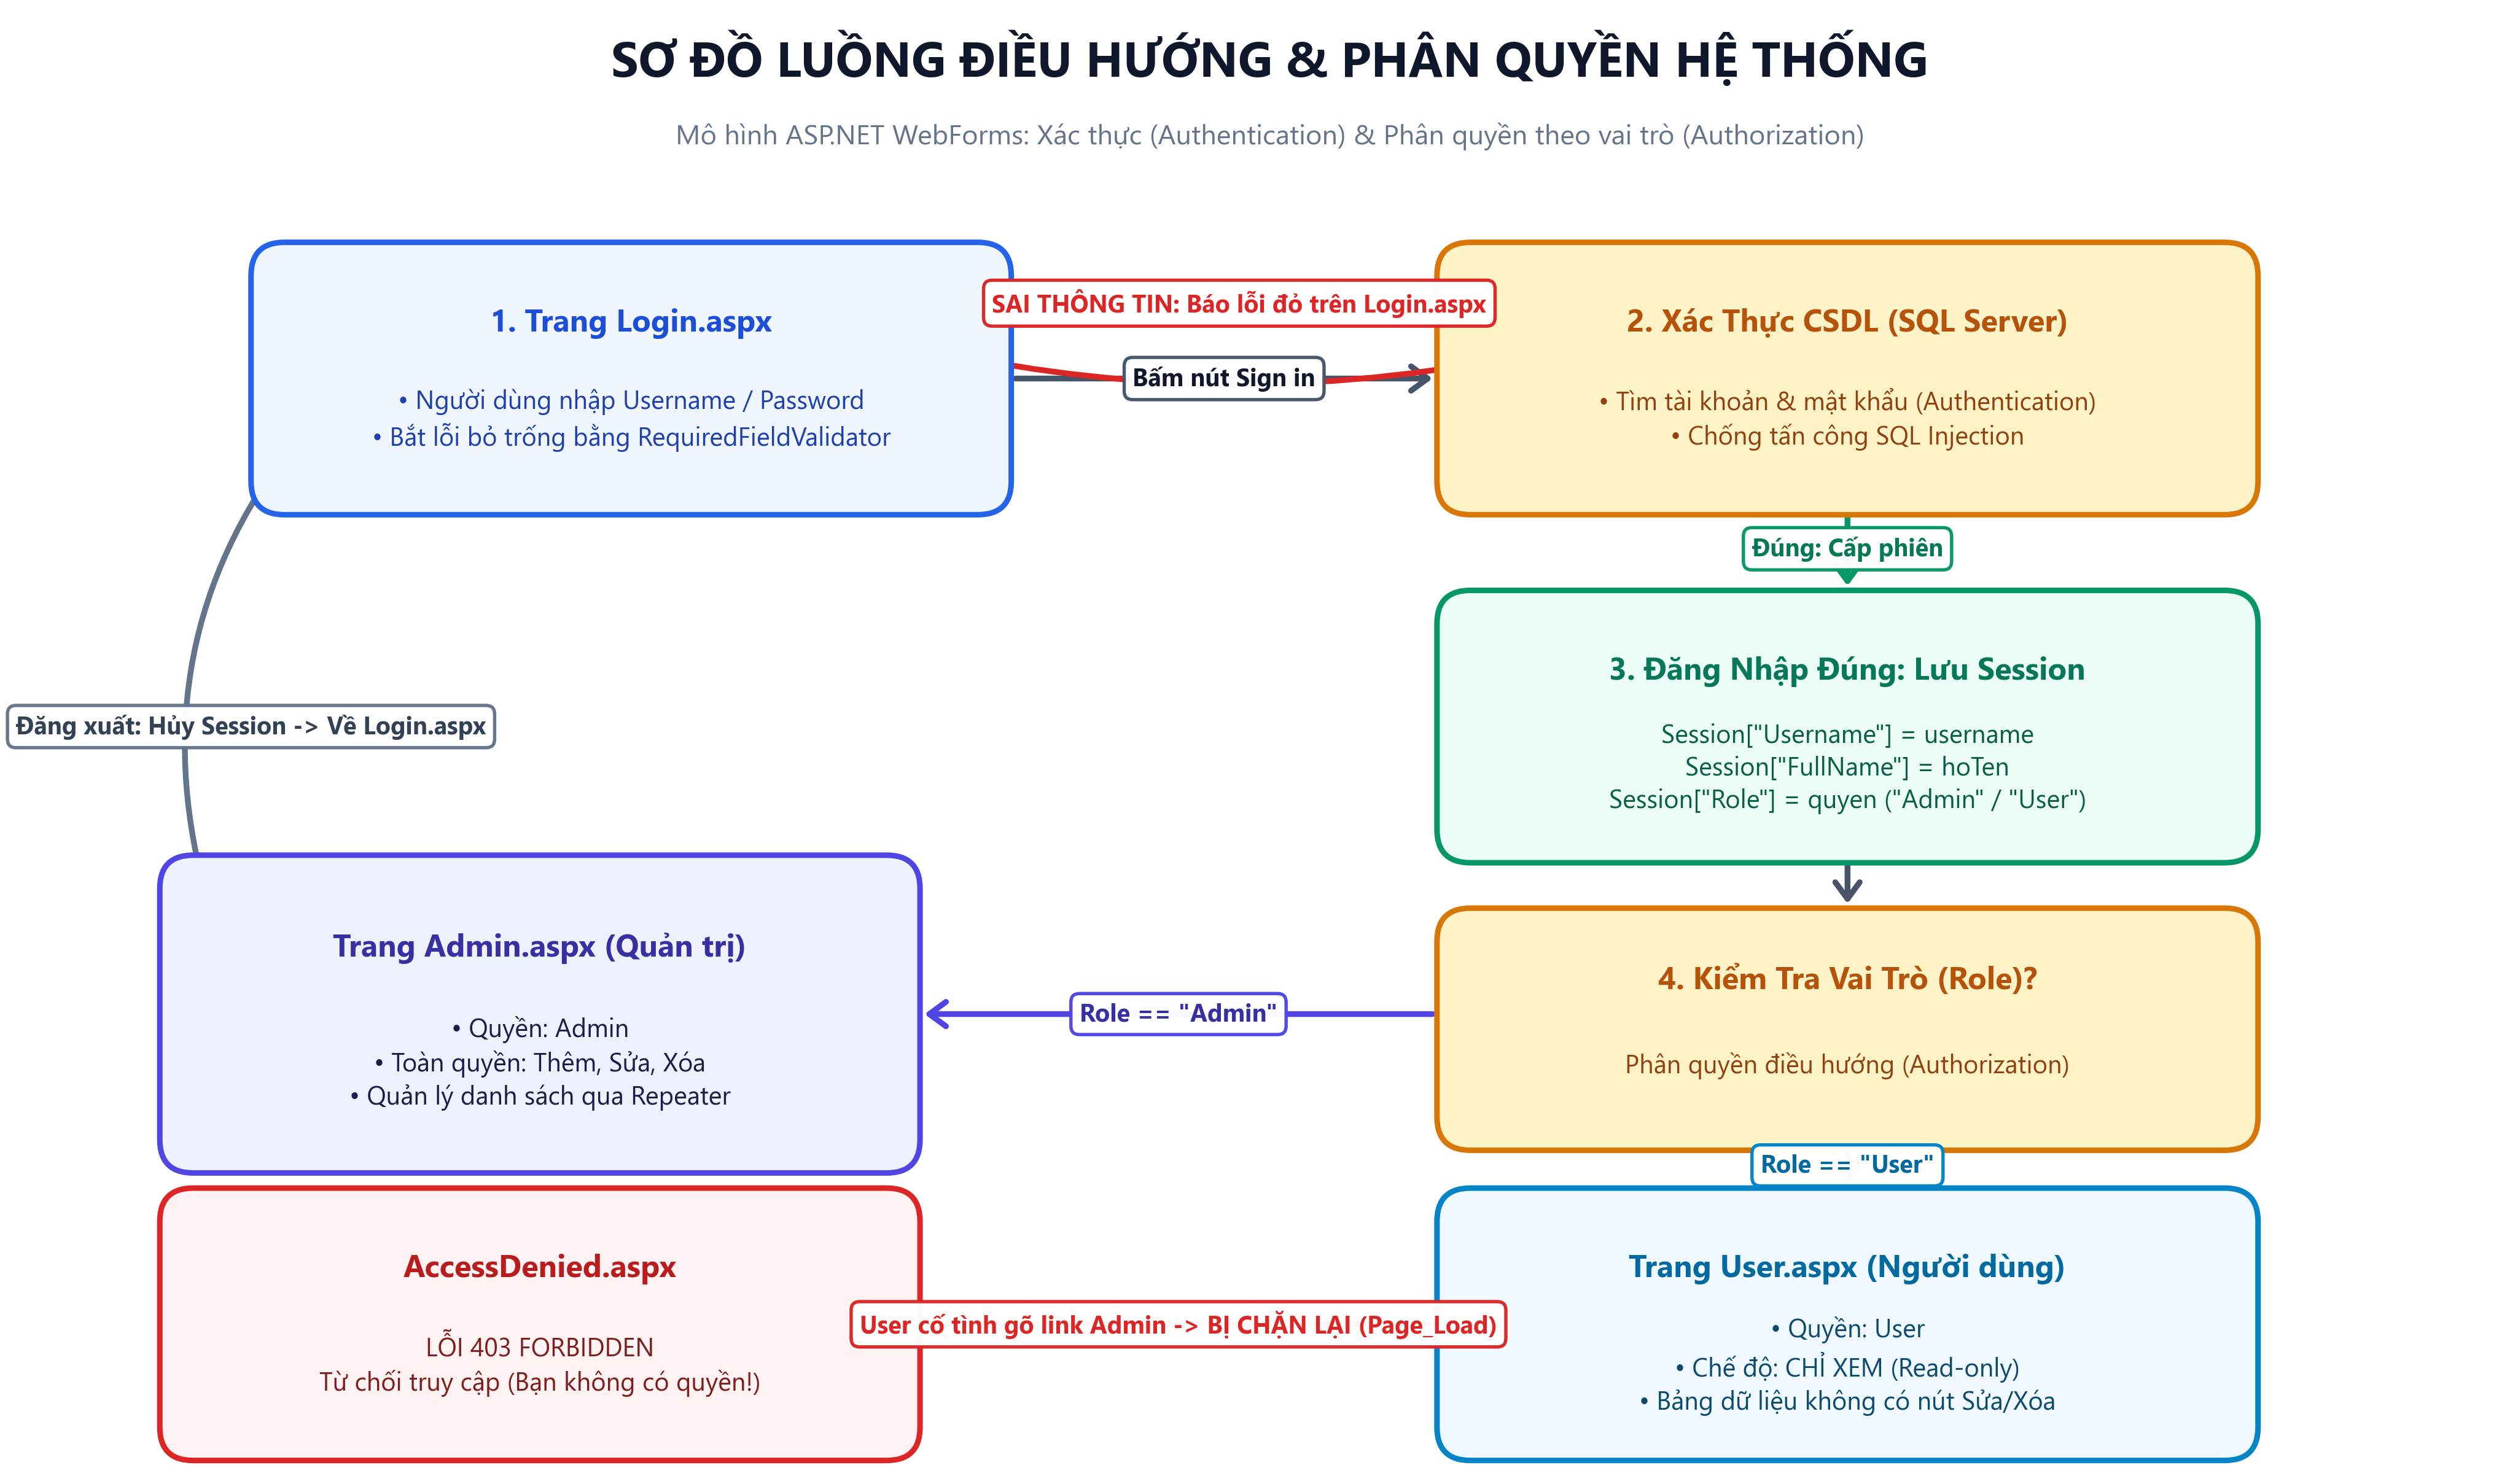
\includegraphics[width=0.95\textwidth]{so_do_dieu_huong_he_thong.png}
\caption{Sơ đồ luồng điều hướng và kiểm soát truy cập hệ thống Login + Role}\label{fig:so_do_dieu_huong}
\end{figure}

\begin{figure}[H]
\centering
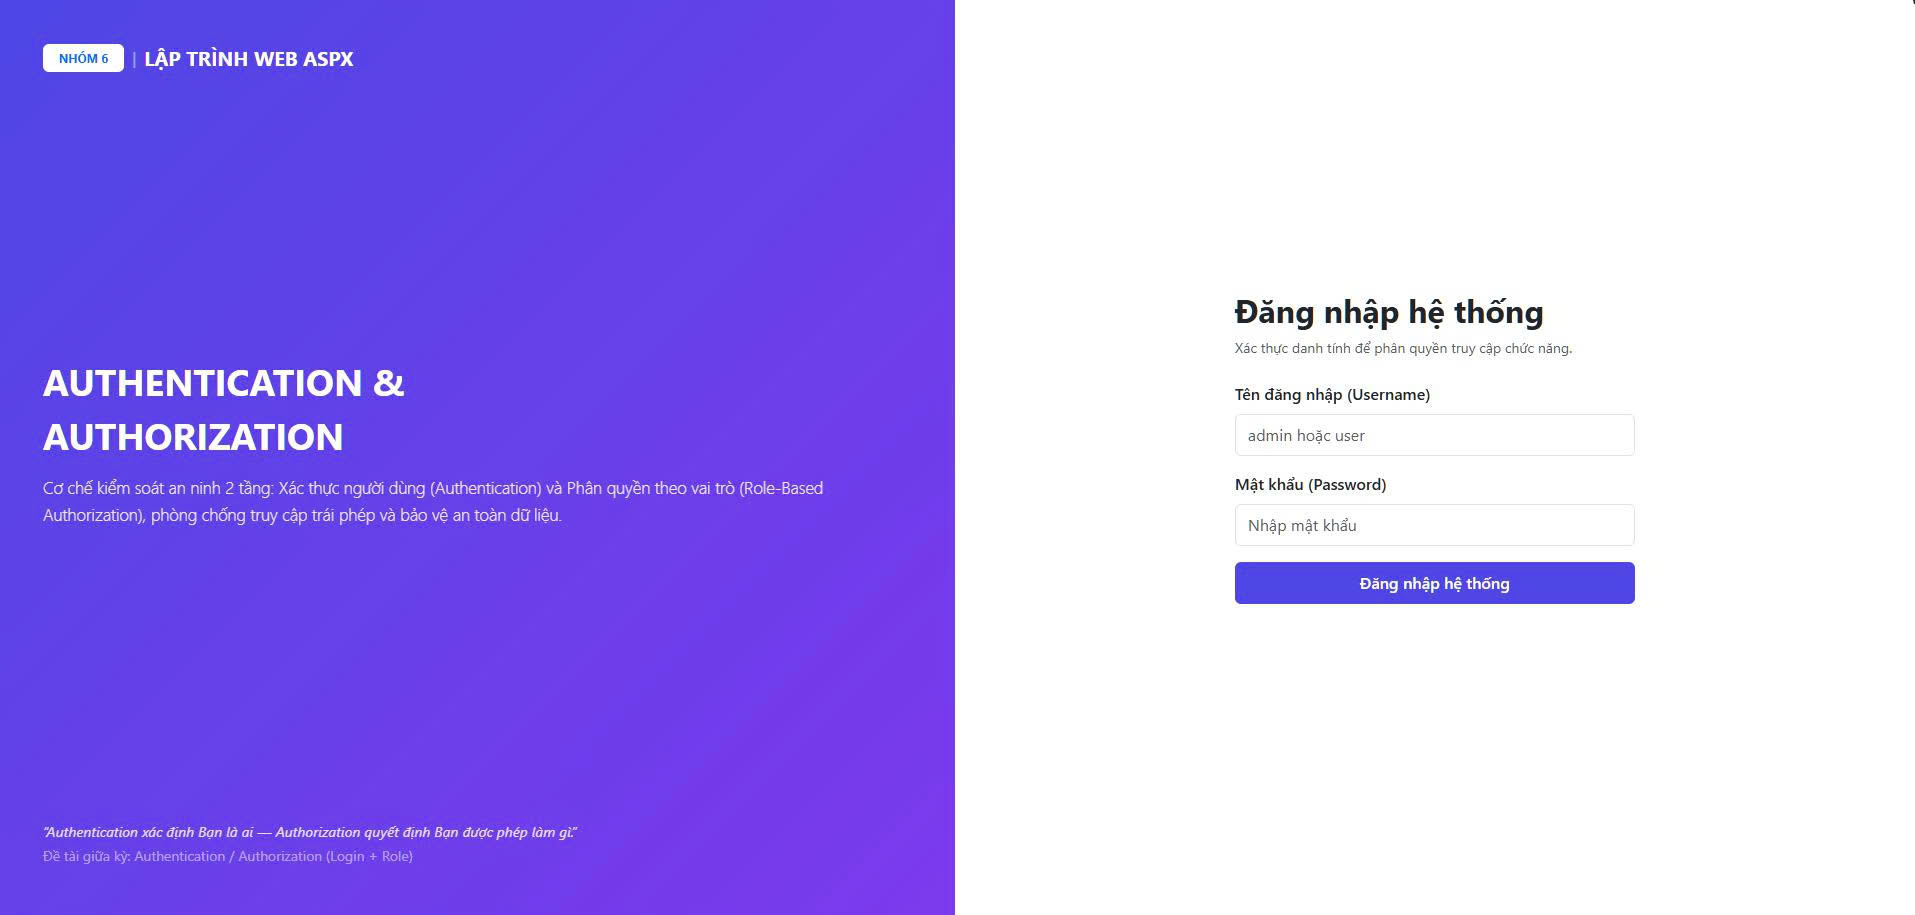
\includegraphics[width=0.92\textwidth]{hinh2_3_login.jpg}
\caption{Giao diện trang Đăng nhập hệ thống (Login.aspx) với Bootstrap 5}\label{fig:ui_login}
\end{figure}

\begin{figure}[H]
\centering
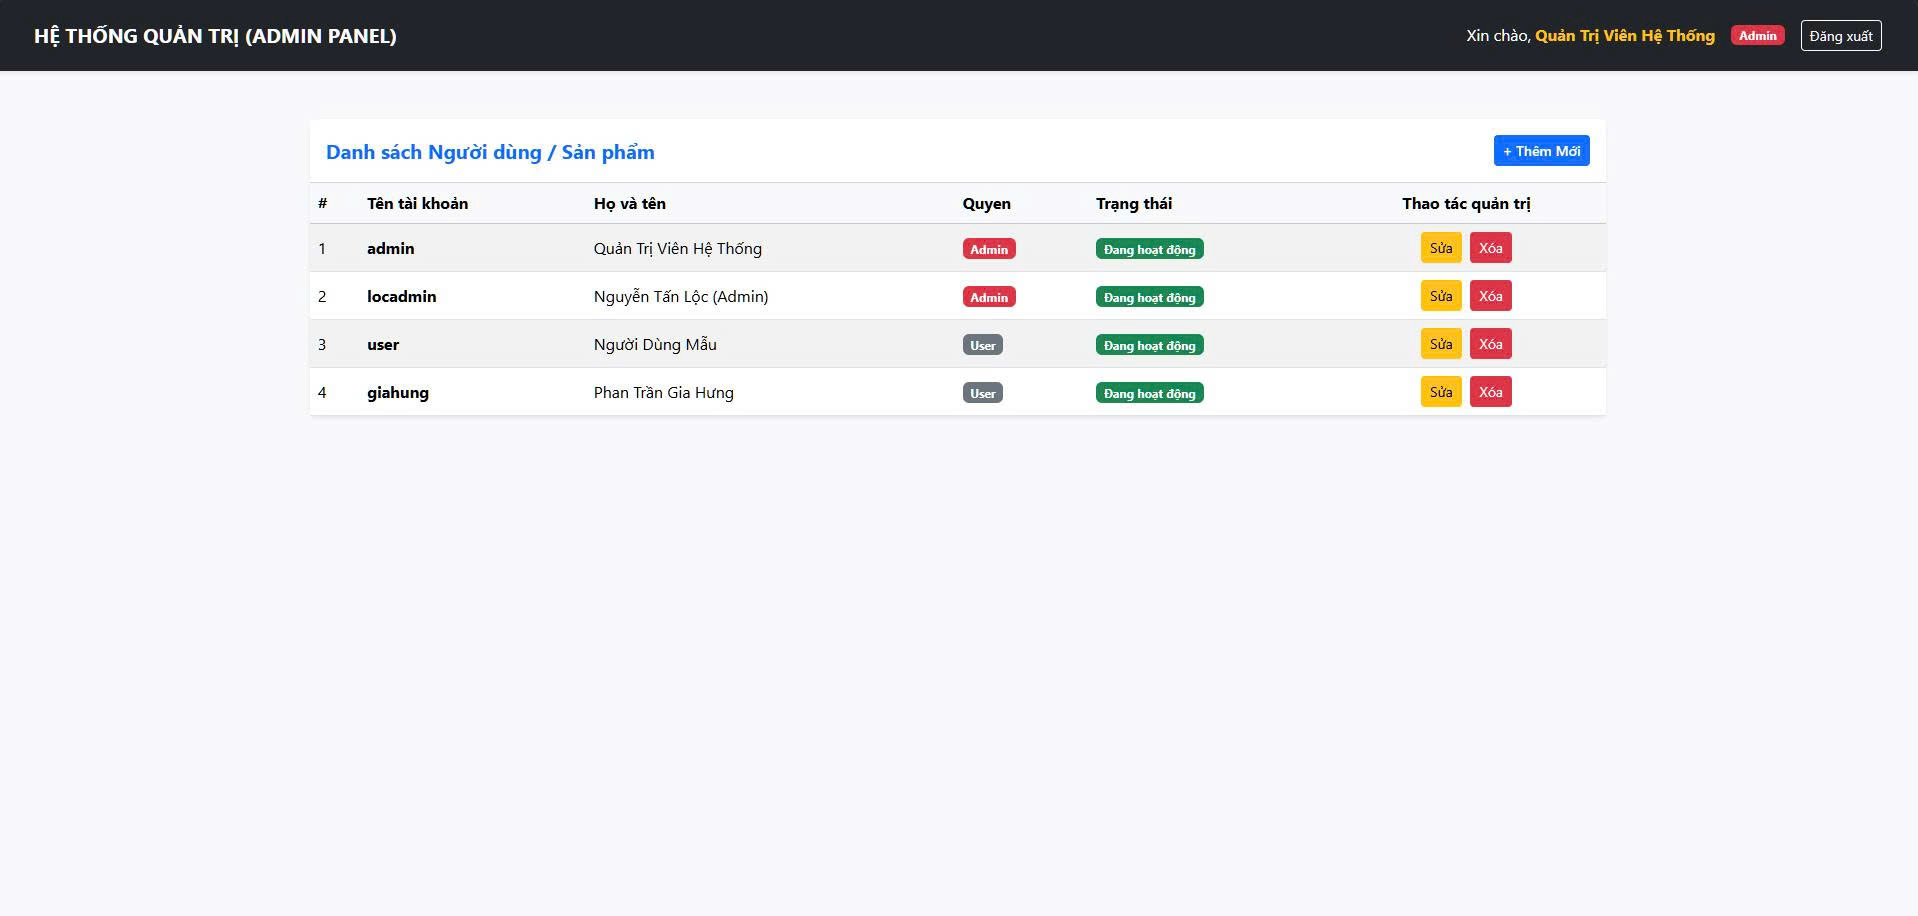
\includegraphics[width=0.92\textwidth]{hinh2_4_admin.jpg}
\caption{Giao diện trang Quản trị (Admin.aspx) với quyền hạn Admin và bảng Repeater}\label{fig:ui_admin}
\end{figure}

\begin{figure}[H]
\centering
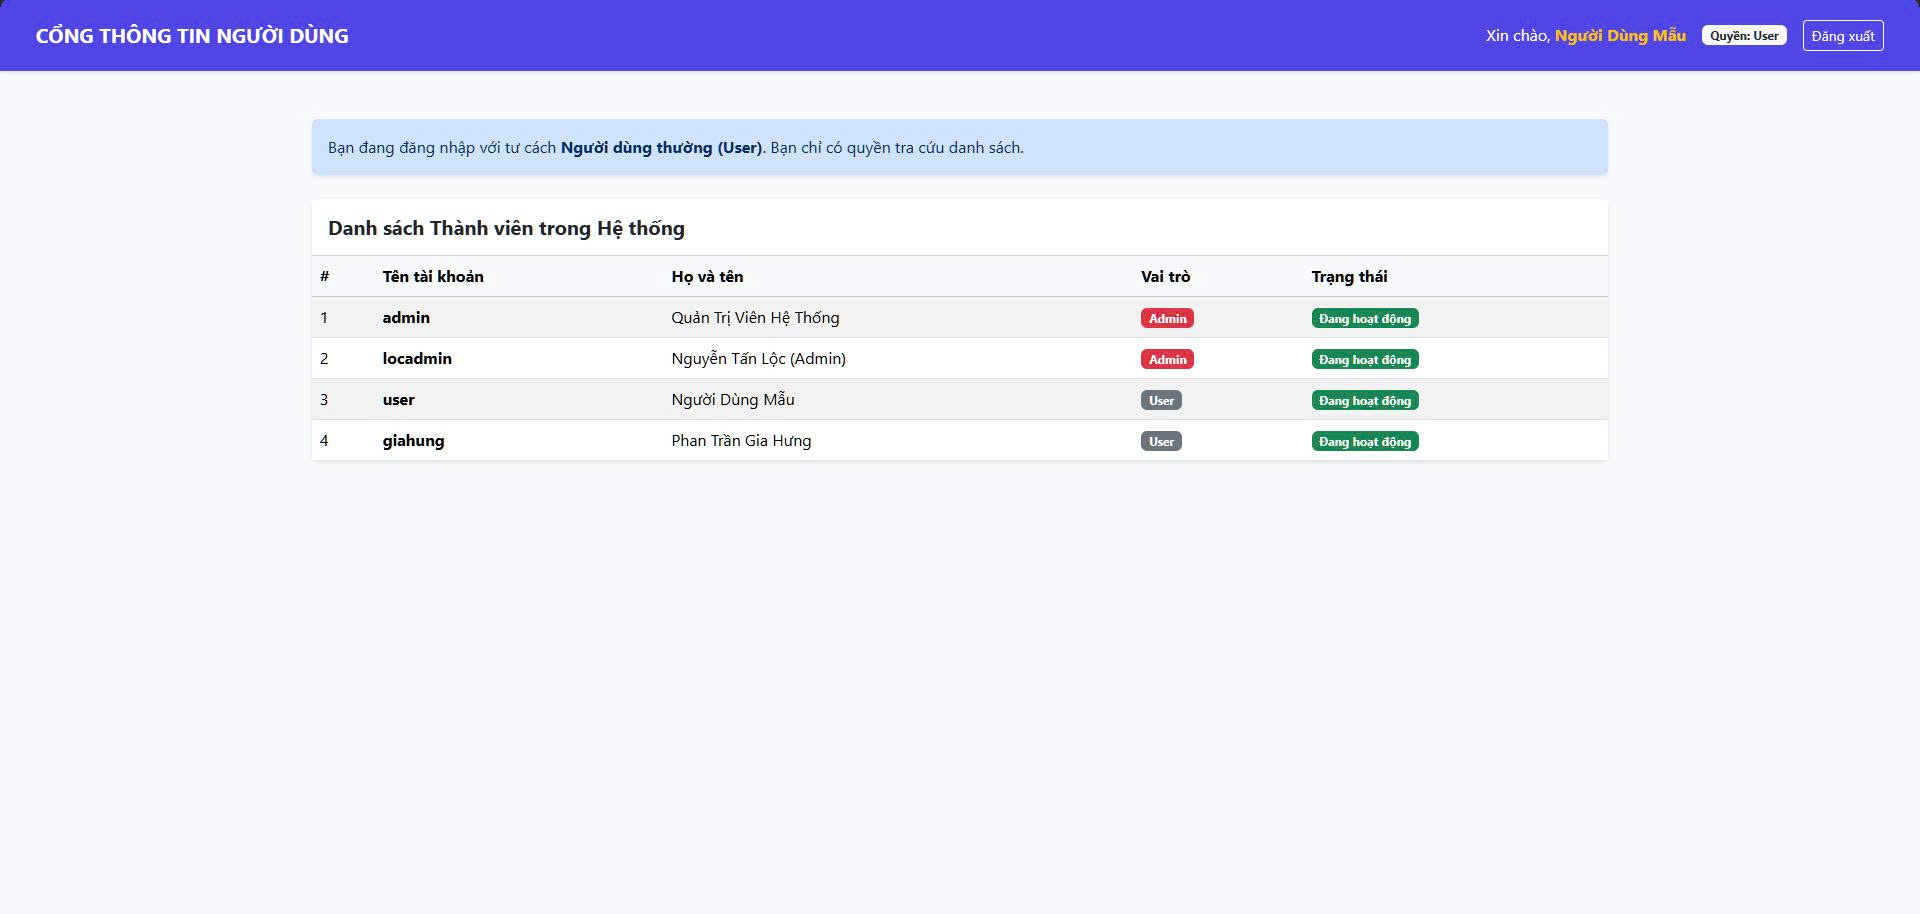
\includegraphics[width=0.92\textwidth]{hinh2_5_user.jpg}
\caption{Giao diện Cổng thông tin người dùng (User.aspx) ở chế độ Chỉ xem (Read-only)}\label{fig:ui_user}
\end{figure}

\begin{figure}[H]
\centering
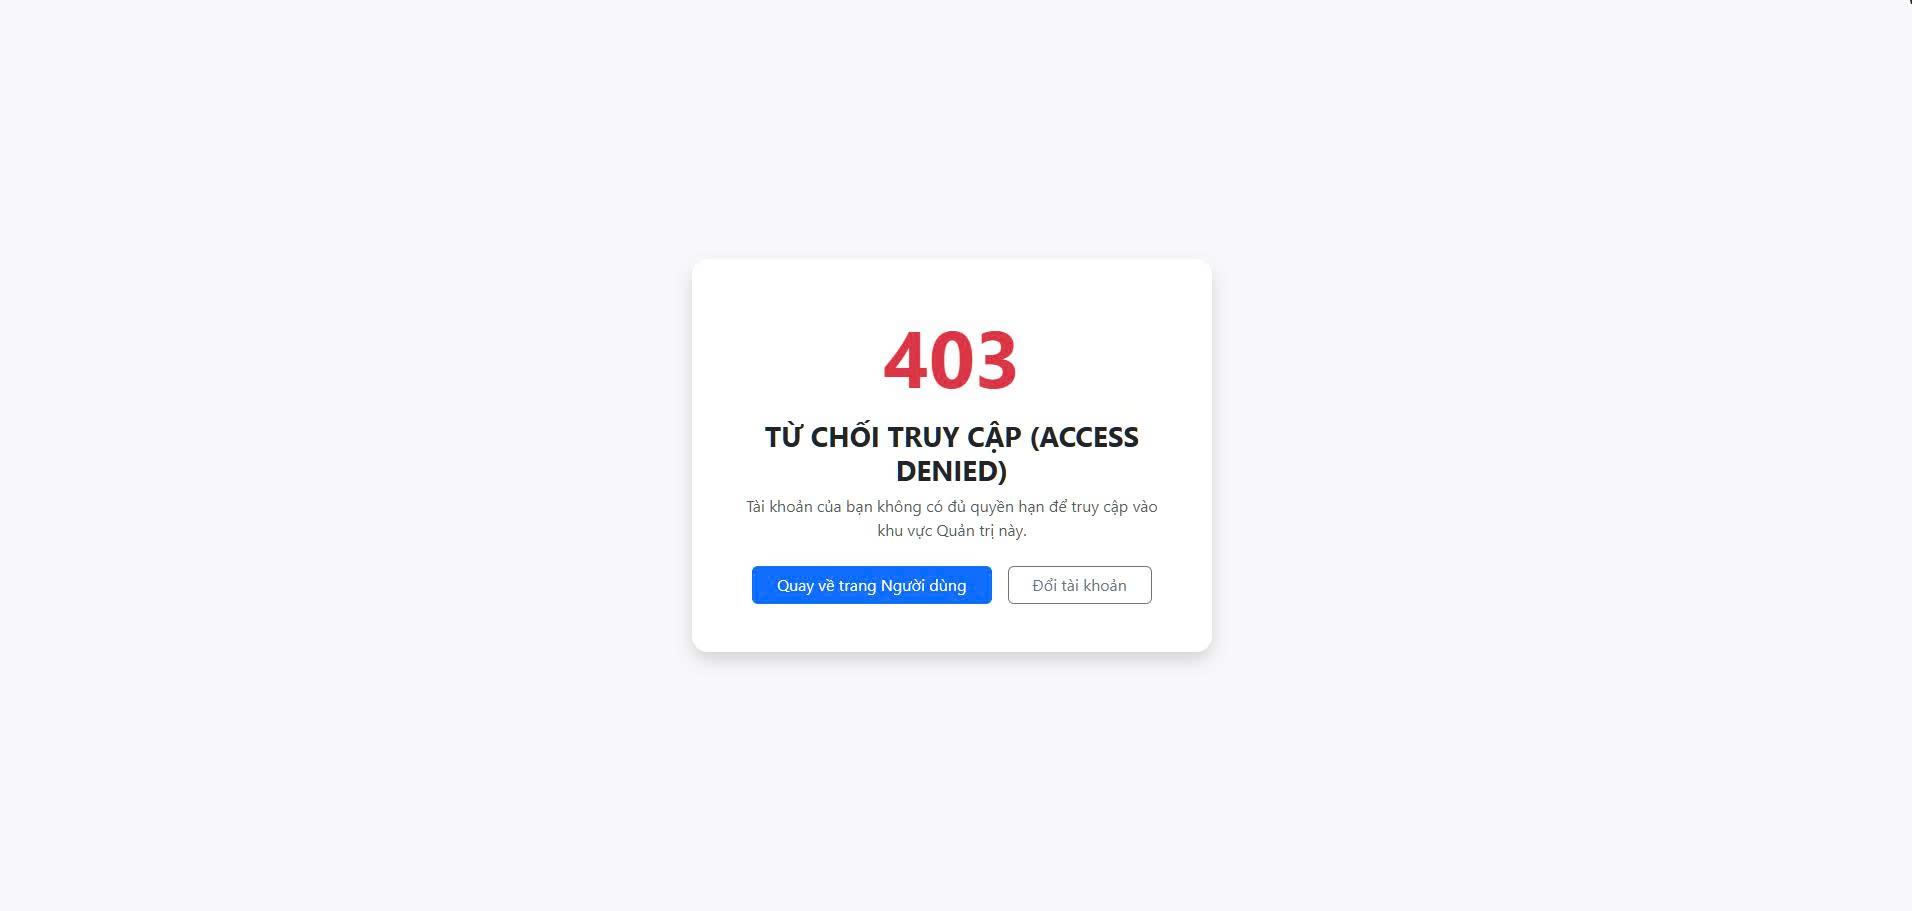
\includegraphics[width=0.82\textwidth]{hinh2_6_access_denied.jpg}
\caption{Giao diện trang Từ chối truy cập 403 Forbidden (AccessDenied.aspx)}\label{fig:ui_accessdenied}
\end{figure}

\section{Lập trình xử lý nghiệp vụ và cài đặt 5 cơ chế phòng thủ an ninh}

\subsection{Cơ chế Đăng nhập an toàn và chống SQL Injection (Login.aspx.cs)}
Khi người dùng nhấn nút 'Đăng nhập', phương thức \texttt{btnLogin\_Click} sẽ thu thập dữ liệu từ \texttt{txtUsername} và \texttt{txtPassword}. Để ngăn chặn triệt để kỹ thuật tấn công SQL Injection (Luồng 3), toàn bộ câu truy vấn được viết dưới dạng Parameterized Query:

\begin{lstlisting}[language={[Sharp]C}, caption={Xử lý đăng nhập bằng Parameterized Query và lưu Session}]
protected void btnLogin_Click(object sender, EventArgs e)
{
    string username = txtUsername.Text.Trim();
    string password = txtPassword.Text.Trim();

    using (SqlConnection conn = new SqlConnection(strConn))
    {
        // DUNG DAU GIU CHO THAM SO @u VA @p THAY VI NOI CHUOI
        string sql = "SELECT HoTen, Quyen FROM NguoiDung WHERE TenDangNhap = @u AND MatKhau = @p";

        using (SqlCommand cmd = new SqlCommand(sql, conn))
        {
            // SQL Server xu ly 100% du lieu nhap vao nhu DU LIEU THUAN (Literal Value)
            // Ky tu nhay don (') va hai gach (--) bi vo hieu hoa hoan toan
            cmd.Parameters.AddWithValue("@u", username);
            cmd.Parameters.AddWithValue("@p", password);

            conn.Open();
            SqlDataReader reader = cmd.ExecuteReader();

            if (reader.Read())
            {
                string hoTen = reader["HoTen"].ToString();
                string quyen = reader["Quyen"].ToString();

                // CHONG TAN CONG CO DINH PHIEN (ANTI SESSION FIXATION)
                Session.Clear(); // Xoa sach session cu truoc khi cap phien moi

                // LUU TRU VAO BO NHO RAM CUA MAY CHU (SERVER-SIDE SESSION)
                Session["Username"] = username;  // Authentication
                Session["FullName"] = hoTen;     // Chao mung
                Session["Role"] = quyen;         // Authorization

                // DIEU HUONG THEO ROLE (PHAN QUYEN)
                if (quyen == "Admin") Response.Redirect("Admin.aspx");
                else Response.Redirect("User.aspx");
            }
            else
            {
                lblThongBao.Text = "Tai khoan hoac mat khau khong chinh xac!";
            }
        }
    }
}
\end{lstlisting}

\subsection{Cơ chế bảo vệ trang chống duyệt URL trực tiếp (Page\_Load)}
Để giải quyết Luồng 1 (Force Browsing) và Luồng 2 (Privilege Escalation), phương thức \texttt{Page\_Load} trong \texttt{Admin.aspx.cs} thiết lập cơ chế kiểm tra bảo mật 2 tầng bắt buộc trước khi thực thi bất kỳ logic nghiệp vụ nào:

\begin{lstlisting}[language={[Sharp]C}, caption={Cơ chế bảo vệ 2 tầng trong Page\_Load của Admin.aspx.cs}]
protected void Page_Load(object sender, EventArgs e)
{
    // ---------------------------------------------------------
    // BUOC 1: KIEM TRA AUTHENTICATION (XAC THUC DANH TINH)
    // ---------------------------------------------------------
    // Neu chua dang nhap (Session["Username"] == null) -> Duoi ngay ve Login.aspx
    if (Session["Username"] == null)
    {
        Response.Redirect("Login.aspx");
        return; // Dung thuc thi toan bo code ben duoi ngay lap tuc!
    }

    // ---------------------------------------------------------
    // BUOC 2: KIEM TRA AUTHORIZATION (PHAN QUYEN TRUY CAP)
    // ---------------------------------------------------------
    // Da dang nhap nhung Role KHONG PHAI "Admin" -> Chan lai va day sang 403
    if (Session["Role"] == null || Session["Role"].ToString() != "Admin")
    {
        Response.Redirect("AccessDenied.aspx");
        return; // Dung thuc thi, tuyet doi khong tai du lieu nhay cam
    }

    if (!IsPostBack)
    {
        lblAdminName.Text = Session["FullName"].ToString();
        LoadDanhSachNguoiDung();
    }
}
\end{lstlisting}

\subsection{Cơ chế vô hiệu hóa Cache trình duyệt và chống nút Back (Anti-BFCache)}
Sau khi Quản trị viên bấm Đăng xuất, Session trên Server đã bị hủy nhưng trình duyệt người dùng (Chrome, Edge) thường lưu trữ ảnh chụp màn hình trong bộ nhớ RAM (BFCache). Khi bấm nút Back, trình duyệt tự rã đông trang cũ mà không gửi request lên Server. Để khắc phục triệt để lỗ hổng này, hệ thống kết hợp giải pháp 2 lớp:
\begin{enumerate}
    \item Lớp Server: Thiết lập đầy đủ các Header HTTP cấm lưu trữ cache trong \texttt{Page\_Load}:
    \begin{lstlisting}[language={[Sharp]C}]
Response.Buffer = true;
Response.ExpiresAbsolute = DateTime.Now.AddDays(-1d);
Response.Expires = -1000;
Response.CacheControl = "no-cache";
Response.Cache.SetCacheability(HttpCacheability.NoCache);
Response.Cache.SetNoStore();
Response.AddHeader("Cache-Control", "no-cache, no-store, must-revalidate, max-age=0");
Response.AddHeader("Pragma", "no-cache");
    \end{lstlisting}
    \item Lớp Client: Đặt đoạn mã JavaScript bắt sự kiện \texttt{pageshow} trong thẻ \texttt{<head>} của \texttt{Admin.aspx} và \texttt{User.aspx}:
\end{enumerate}

\begin{lstlisting}[language=HTML, caption={Script chống BFCache phía Client}]
<script type="text/javascript">
    // PHONG THU LUONG 4: CHONG HIEN THI LAI TRANG KHI BAM NUT "BACK" (BFCACHE)
    window.addEventListener("pageshow", function (event) {
        var isBack = event.persisted || 
            (window.performance && window.performance.navigation && window.performance.navigation.type === 2) ||
            (window.performance && window.performance.getEntriesByType && window.performance.getEntriesByType("navigation")[0] && window.performance.getEntriesByType("navigation")[0].type === "back_forward");

        if (isBack) {
            // Ep trinh duyet gui request len Server -> Page_Load da ve Login ngay
            window.location.reload();
        }
    });
</script>
\end{lstlisting}

\subsection{Xử lý Đăng xuất an toàn và hủy toàn bộ phiên làm việc (Logout.aspx.cs)}
Khi người dùng nhấn nút 'Đăng xuất' (hoặc truy cập trực tiếp trang \texttt{Logout.aspx}), hệ thống thực thi chuỗi hành động hủy phiên làm việc triệt để:

\begin{lstlisting}[language={[Sharp]C}, caption={Xử lý hủy phiên làm việc triệt để khi Đăng xuất}]
protected void btnLogout_Click(object sender, EventArgs e)
{
    // 1. Xoa sach moi bien luu trong bo nho Session tren may chu
    Session.Clear();

    // 2. Huy bo hoan toan dinh danh phien hien tai tren Web Server RAM
    Session.Abandon();

    // 3. Xoa cookie dinh danh phien ASP.NET_SessionId tren may khach
    if (Request.Cookies["ASP.NET_SessionId"] != null)
    {
        Response.Cookies["ASP.NET_SessionId"].Value = string.Empty;
        Response.Cookies["ASP.NET_SessionId"].Expires = DateTime.Now.AddMonths(-20);
    }

    // 4. Chuyen nguoi dung quay ve trang Dang nhap
    Response.Redirect("Login.aspx");
}
\end{lstlisting}

\section{Hướng dẫn thực hành cho lớp (Kịch bản 5 tiết thực hành)}
Theo yêu cầu của học phần, nhóm báo cáo có nhiệm vụ chủ trì và hướng dẫn toàn thể sinh viên trong lớp thực hành trong thời lượng 5 tiết học. Để buổi thực hành đạt hiệu quả cao nhất và không làm mất thời gian vào các khâu dựng giao diện, nhóm đã chuẩn bị gói bài tập chuyên biệt \texttt{SEMI\_FINAL\_ASPX\_Starter.zip}:
\begin{itemize}
    \item \textbf{Cấu trúc gói bài tập Starter:} Đã dựng sẵn toàn bộ CSDL, trang Login.aspx, giao diện Bootstrap 5 cho Admin.aspx và User.aspx. Hai khối mã nguồn kiểm tra Authentication và Authorization tại Page\_Load đã được xóa đi và để sẵn các dòng ghi chú hướng dẫn.
    \item \textbf{Nhiệm vụ của sinh viên dưới lớp:} Dưới sự hướng dẫn của nhóm, các bạn sinh viên sẽ tự tay mở Visual Studio và điền đúng 2 khối code bảo mật:
    \begin{enumerate}
        \item Viết khối kiểm tra Authentication trong \texttt{User.aspx.cs} và \texttt{Admin.aspx.cs}.
        \item Viết khối kiểm tra Authorization phân quyền Admin trong \texttt{Admin.aspx.cs}.
    \end{enumerate}
\end{itemize}

Tiêu chí đánh giá và Rubric chấm điểm bài thực hành 5 tiết cho sinh viên trong lớp được quy định cụ thể như sau:

\begin{table}[H]
\centering
\small
\renewcommand{\arraystretch}{1.12}
\begin{tabularx}{\textwidth}{>{\raggedright\arraybackslash}p{3.2cm} >{\raggedright\arraybackslash}X >{\centering\arraybackslash}p{2.0cm} >{\raggedright\arraybackslash}p{3.5cm}}
\toprule
\textbf{Tiêu chí đánh giá} & \textbf{Mô tả yêu cầu kỹ thuật} & \textbf{Điểm chuẩn} & \textbf{Kết quả nghiệm thu} \\
\midrule
1. Cài đặt CSDL \& Dự án & Nạp thành công database.sql vào SQL Server, mở được solution trong Visual Studio không lỗi biên dịch & 2.0 điểm & Chạy được trang Login \\
\addlinespace
2. Hoàn thiện Authentication & Tự viết đúng đoạn code kiểm tra Session['Username'] == null, chặn được Force Browsing về Login.aspx & 3.0 điểm & Chặn người lạ gõ URL \\
\addlinespace
3. Hoàn thiện Authorization & Tự viết đúng đoạn code kiểm tra Session['Role'] != 'Admin', chặn được tài khoản User sang AccessDenied.aspx & 3.0 điểm & Hiện lỗi 403 khi vào Admin \\
\addlinespace
4. Kiểm thử Đăng xuất \& Cache & Kiểm thử bấm nút Đăng xuất và bấm nút Back trình duyệt, chứng minh hệ thống không bị xem lén dữ liệu & 1.0 điểm & Đẩy về Login khi bấm Back \\
\addlinespace
5. Thao tác và Tác phong & Thao tác thành thạo, trả lời được câu hỏi vấn đáp ngắn về sự khác biệt giữa Authentication và Authorization & 1.0 điểm & Hiểu bản chất vấn đề \\
\bottomrule
\end{tabularx}
\caption{Tiêu chí đánh giá và Rubric chấm điểm bài thực hành phân quyền 5 tiết}\label{tab:rubric_danhgia}
\end{table}

\section{Kịch bản kiểm thử an ninh hệ thống (5 Test Cases thực nghiệm)}
Để chứng minh tính đúng đắn và khả năng phòng thủ toàn diện của hệ thống, nhóm thực hiện quy trình kiểm thử với 5 kịch bản thực nghiệm:

\begin{table}[H]
\centering
\footnotesize
\renewcommand{\arraystretch}{1.25}
\begin{tabularx}{\textwidth}{>{\raggedright\arraybackslash}p{2.5cm} >{\raggedright\arraybackslash}p{2.3cm} >{\raggedright\arraybackslash}p{3.6cm} >{\raggedright\arraybackslash}X >{\centering\arraybackslash}p{1.8cm}}
\toprule
\textbf{Kịch bản kiểm thử} & \textbf{Mục tiêu kiểm tra} & \textbf{Thao tác thực nghiệm} & \textbf{Kết quả thực tế} & \textbf{Đánh giá} \\
\midrule
\textbf{Kịch bản 1: Force Browsing} & Kiểm tra Authentication khi chưa đăng nhập & Mở tab ẩn danh, gõ trực tiếp URL:\newline \texttt{.../Admin.aspx}\newline rồi nhấn phím Enter & Phát hiện Session null, chuyển hướng (Redirect 302) về Login.aspx. Tuyệt đối không lộ dữ liệu & \textbf{\color{green!60!black}ĐẠT\newline(PASS)} \\
\addlinespace
\textbf{Kịch bản 2: Privilege Escalation} & Kiểm tra Authorization phân quyền vai trò & Đăng nhập User thường $\rightarrow$ Vào User.aspx. Sửa URL thành Admin.aspx rồi Enter & Nhận thấy Session['Role'] != 'Admin'. Lập tức đá sang AccessDenied.aspx (Mã lỗi 403) & \textbf{\color{green!60!black}ĐẠT\newline(PASS)} \\
\addlinespace
\textbf{Kịch bản 3: SQL Injection} & Khả năng bảo vệ của Parameterized Query & Tên đăng nhập: \texttt{admin' --}\newline Mật khẩu: gõ tùy ý\newline rồi bấm nút Đăng nhập & Thông báo lỗi đỏ: \textit{'Tài khoản hoặc mật khẩu không chính xác!'}. Không thể vượt mặt & \textbf{\color{green!60!black}ĐẠT\newline(PASS)} \\
\addlinespace
\textbf{Kịch bản 4: Anti-BFCache Back Button} & Vô hiệu hóa Cache trình duyệt sau Logout & Đăng nhập Admin $\rightarrow$ Bấm 'Đăng xuất' $\rightarrow$ Bấm nút mũi tên Back ($\leftarrow$) trình duyệt & Sự kiện \texttt{pageshow} phát hiện cache, ép reload. Server thấy Session null nên đá về Login & \textbf{\color{green!60!black}ĐẠT\newline(PASS)} \\
\addlinespace
\textbf{Kịch bản 5: DOM Tampering F12} & Nguyên tắc Quyền tối thiểu \& Double-Check & Đăng nhập quyền User $\rightarrow$ Nhấn F12 kiểm tra mã nguồn HTML của bảng & HTML không hề sinh nút Sửa/Xóa của Admin. Mọi request giả mạo bị chặn ở Server & \textbf{\color{green!60!black}ĐẠT\newline(PASS)} \\
\bottomrule
\end{tabularx}
\caption{Kết quả kiểm thử an ninh 5 kịch bản thực tế}\label{tab:test_cases}
\end{table}

% ==========================================
% PHỤ LỤC
% ==========================================
\appendix
\chapter*{PHỤ LỤC: MÃ NGUỒN HOÀN CHỈNH}
\addcontentsline{toc}{chapter}{PHỤ LỤC: MÃ NGUỒN HOÀN CHỈNH}

\section*{Phụ lục A: Kịch bản Cơ sở dữ liệu (database.sql)}
\addcontentsline{toc}{section}{Phụ lục A: Kịch bản Cơ sở dữ liệu (database.sql)}
\begin{lstlisting}[language=SQL]
IF NOT EXISTS (SELECT * FROM sys.databases WHERE name = 'QL_NguoiDung')
BEGIN
    CREATE DATABASE QL_NguoiDung;
END
GO
USE QL_NguoiDung;
GO

IF NOT EXISTS (SELECT * FROM sys.tables WHERE name = 'NguoiDung')
BEGIN
    CREATE TABLE NguoiDung (
        Id INT IDENTITY(1,1) PRIMARY KEY,
        TenDangNhap VARCHAR(50) NOT NULL UNIQUE,
        MatKhau VARCHAR(50) NOT NULL,
        HoTen NVARCHAR(100) NOT NULL,
        Email VARCHAR(100),
        Quyen VARCHAR(20) NOT NULL, -- 'Admin' hoac 'User'
        TrangThai NVARCHAR(30) DEFAULT N'Dang hoat dong'
    );
END
GO

INSERT INTO NguoiDung (TenDangNhap, MatKhau, HoTen, Email, Quyen, TrangThai) VALUES
('admin', '123', N'Quan Tri Vien He Thong', 'admin@dthu.edu.vn', 'Admin', N'Dang hoat dong'),
('locadmin', '123', N'Nguyen Tan Loc (Admin)', 'tanloc@dthu.edu.vn', 'Admin', N'Dang hoat dong'),
('user', '123', N'Nguoi Dung Mau', 'user@dthu.edu.vn', 'User', N'Dang hoat dong'),
('giahung', '123', N'Phan Tran Gia Hung', 'giahung@dthu.edu.vn', 'User', N'Dang hoat dong'),
('vanan', '123', N'Tran Van An', 'vanan@dthu.edu.vn', 'User', N'Dang hoat dong'),
('thuhuong', '123', N'Le Thi Thu Huong', 'thuhuong@dthu.edu.vn', 'User', N'Dang hoat dong');
GO
\end{lstlisting}

\section*{Phụ lục B: Mã nguồn giao diện Quản trị (Admin.aspx)}
\addcontentsline{toc}{section}{Phụ lục B: Mã nguồn giao diện Quản trị (Admin.aspx)}
\begin{lstlisting}[language=HTML]
<%@ Page Language="C#" AutoEventWireup="true" CodeBehind="Admin.aspx.cs" Inherits="SEMI_FINAL_ASPX.Admin" %>
<!DOCTYPE html>
<html xmlns="http://www.w3.org/1999/xhtml">
<head runat="server">
    <meta charset="utf-8" />
    <title>Trang Quan Tri - Admin Panel</title>
    <link href="Content/bootstrap.min.css" rel="stylesheet" />
    <script type="text/javascript">
        window.addEventListener("pageshow", function (event) {
            var isBack = event.persisted || 
                (window.performance && window.performance.navigation && window.performance.navigation.type === 2) ||
                (window.performance && window.performance.getEntriesByType && window.performance.getEntriesByType("navigation")[0] && window.performance.getEntriesByType("navigation")[0].type === "back_forward");
            if (isBack) { window.location.reload(); }
        });
    </script>
</head>
<body class="bg-light">
    <form id="form1" runat="server">
        <nav class="navbar navbar-expand-lg navbar-dark bg-dark px-4 py-3 shadow-sm">
            <div class="container-fluid">
                <span class="navbar-brand fw-bold text-uppercase">He Thong Quan Tri (Admin Panel)</span>
                <div class="d-flex align-items-center gap-3">
                    <span class="text-white">Xin chao, <asp:Label ID="lblAdminName" runat="server" CssClass="fw-bold text-warning"></asp:Label></span>
                    <span class="badge bg-danger px-2 py-1">Admin</span>
                    <asp:Button ID="btnLogout" runat="server" Text="Dang xuat" CssClass="btn btn-outline-light btn-sm" OnClick="btnLogout_Click" />
                </div>
            </div>
        </nav>
        <div class="container my-5">
            <div class="card shadow-sm border-0 rounded-3">
                <div class="card-header bg-white py-3 d-flex justify-content-between align-items-center">
                    <h5 class="mb-0 fw-bold text-primary">Danh sach Nguoi dung trong He thong</h5>
                    <button type="button" class="btn btn-primary btn-sm fw-semibold">+ Them Moi</button>
                </div>
                <div class="card-body p-0">
                    <asp:Repeater ID="rptNguoiDung" runat="server">
                        <HeaderTemplate>
                            <table class="table table-hover table-striped mb-0 align-middle">
                                <thead class="table-light">
                                    <tr>
                                        <th>#</th>
                                        <th>Ten tai khoan</th>
                                        <th>Ho va ten</th>
                                        <th>Quyen</th>
                                        <th>Trang thai</th>
                                        <th class="text-center">Thao tac quan tri</th>
                                    </tr>
                                </thead>
                                <tbody>
                        </HeaderTemplate>
                        <ItemTemplate>
                            <tr>
                                <td><%# Container.ItemIndex + 1 %></td>
                                <td><strong><%# Eval("TenDangNhap") %></strong></td>
                                <td><%# Eval("HoTen") %></td>
                                <td>
                                    <span class='badge <%# Eval("Quyen").ToString() == "Admin" ? "bg-danger" : "bg-secondary" %>'>
                                        <%# Eval("Quyen") %>
                                    </span>
                                </td>
                                <td><span class="badge bg-success"><%# Eval("TrangThai") %></span></td>
                                <td class="text-center">
                                    <button type="button" class="btn btn-warning btn-sm me-1">Sua</button>
                                    <button type="button" class="btn btn-danger btn-sm">Xoa</button>
                                </td>
                            </tr>
                        </ItemTemplate>
                        <FooterTemplate>
                                </tbody>
                            </table>
                        </FooterTemplate>
                    </asp:Repeater>
                </div>
            </div>
        </div>
    </form>
</body>
</html>
\end{lstlisting}

\section*{Phụ lục C: Mã nguồn xử lý máy chủ (Admin.aspx.cs)}
\addcontentsline{toc}{section}{Phụ lục C: Mã nguồn xử lý máy chủ (Admin.aspx.cs)}
\begin{lstlisting}[language={[Sharp]C}]
using System;
using System.Configuration;
using System.Data;
using System.Data.SqlClient;
using System.Web;
using System.Web.UI;

namespace SEMI_FINAL_ASPX
{
    public partial class Admin : System.Web.UI.Page
    {
        private string strConn = ConfigurationManager.ConnectionStrings["QLNguoiDungConn"].ConnectionString;

        protected void Page_Load(object sender, EventArgs e)
        {
            // VO HIEU HOA CACHE TRINH DUYET (CHONG NUT BACK SAU LOGOUT)
            Response.Buffer = true;
            Response.ExpiresAbsolute = DateTime.Now.AddDays(-1d);
            Response.Expires = -1000;
            Response.CacheControl = "no-cache";
            Response.Cache.SetCacheability(HttpCacheability.NoCache);
            Response.Cache.SetNoStore();
            Response.Cache.SetExpires(DateTime.UtcNow.AddMinutes(-1));
            Response.AddHeader("Cache-Control", "no-cache, no-store, must-revalidate, max-age=0");
            Response.AddHeader("Pragma", "no-cache");

            // BUOC 1: KIEM TRA AUTHENTICATION
            if (Session["Username"] == null)
            {
                Response.Redirect("Login.aspx");
                return;
            }

            // BUOC 2: KIEM TRA AUTHORIZATION
            if (Session["Role"] == null || Session["Role"].ToString() != "Admin")
            {
                Response.Redirect("AccessDenied.aspx");
                return;
            }

            if (!IsPostBack)
            {
                lblAdminName.Text = Session["FullName"] != null ? Session["FullName"].ToString() : Session["Username"].ToString();
                LoadDanhSachNguoiDung();
            }
        }

        private void LoadDanhSachNguoiDung()
        {
            using (SqlConnection conn = new SqlConnection(strConn))
            {
                string sql = "SELECT Id, TenDangNhap, HoTen, Quyen, TrangThai FROM NguoiDung";
                using (SqlDataAdapter da = new SqlDataAdapter(sql, conn))
                {
                    DataTable dt = new DataTable();
                    da.Fill(dt);
                    rptNguoiDung.DataSource = dt;
                    rptNguoiDung.DataBind();
                }
            }
        }

        protected void btnLogout_Click(object sender, EventArgs e)
        {
            Session.Clear();
            Session.Abandon();
            if (Request.Cookies["ASP.NET_SessionId"] != null)
            {
                Response.Cookies["ASP.NET_SessionId"].Value = string.Empty;
                Response.Cookies["ASP.NET_SessionId"].Expires = DateTime.Now.AddMonths(-20);
            }
            Response.Redirect("Login.aspx");
        }
    }
}
\end{lstlisting}

\end{document}
